\subsubsection{Bestimmung der Reibungskonstanten}

Die Reibungskonstante kann über folgende DGL berechnet werden.
Die Summe der Drehmomente ergibt sich aus dem Drehmoment $M_m$
abzüglich des Reibungsdrehmoments $M_R$ und des Lastdrehmoments.
Diese sind gleich der zeitlichen Änderung der Winkelgeschwindikeit 
$\frac{d \omega}{dt}$ multipliziert mit dem Trägheitsmoment $J$.

\begin{equation} \label{eq221}
    \begin{split}
        J \frac{d \omega}{d t} &= \sum M = M_m - M_R - M_L \\
        J \frac{d \omega}{d t} &= \sum M = k_m \cdot i(t) - c_r \omega (t) - M_L 
    \end{split}
\end{equation}

Um die Reibungskonstante $c_r$ nun zu bestimmen, ist es günstig das
System im Leerlauf zu betrachten, da $M_L=0$ und nach Abklingen des
Einschaltvorgangs $\frac{d\omega}{dt} =0$. Aus der DGL ergibt sich
folgende einfache Gleichung.

\begin{equation} \label{eq222}
    \begin{split}
        0 & = k_m \cdot i(t) - c_r \omega (t)
    \end{split}
\end{equation}

Daraus ergibt sich folgende Funktion.

\begin{equation} \label{eq222}
    \begin{split}
        \omega = f_3(i) = \frac{k_m}{c_r} i
    \end{split}
\end{equation}

Nun kann mittels der linearen Regression aus den beiden Vektoren die Steigung
$m$ bestimmt werden, aus der sich die Reibungskonstante $c_r$ berechnen lässt.

\begin{equation} \label{eq218}
    \begin{split}
       m &=  \frac{k_m}{c_r}\\
       c_r &= \frac{k_m}{m} \simeq 3,24 \cdot 10^{-9} \mathrm{\frac{Nm s}{rad}}
    \end{split}
\end{equation}

\begin{figure}[H]
 \centering
    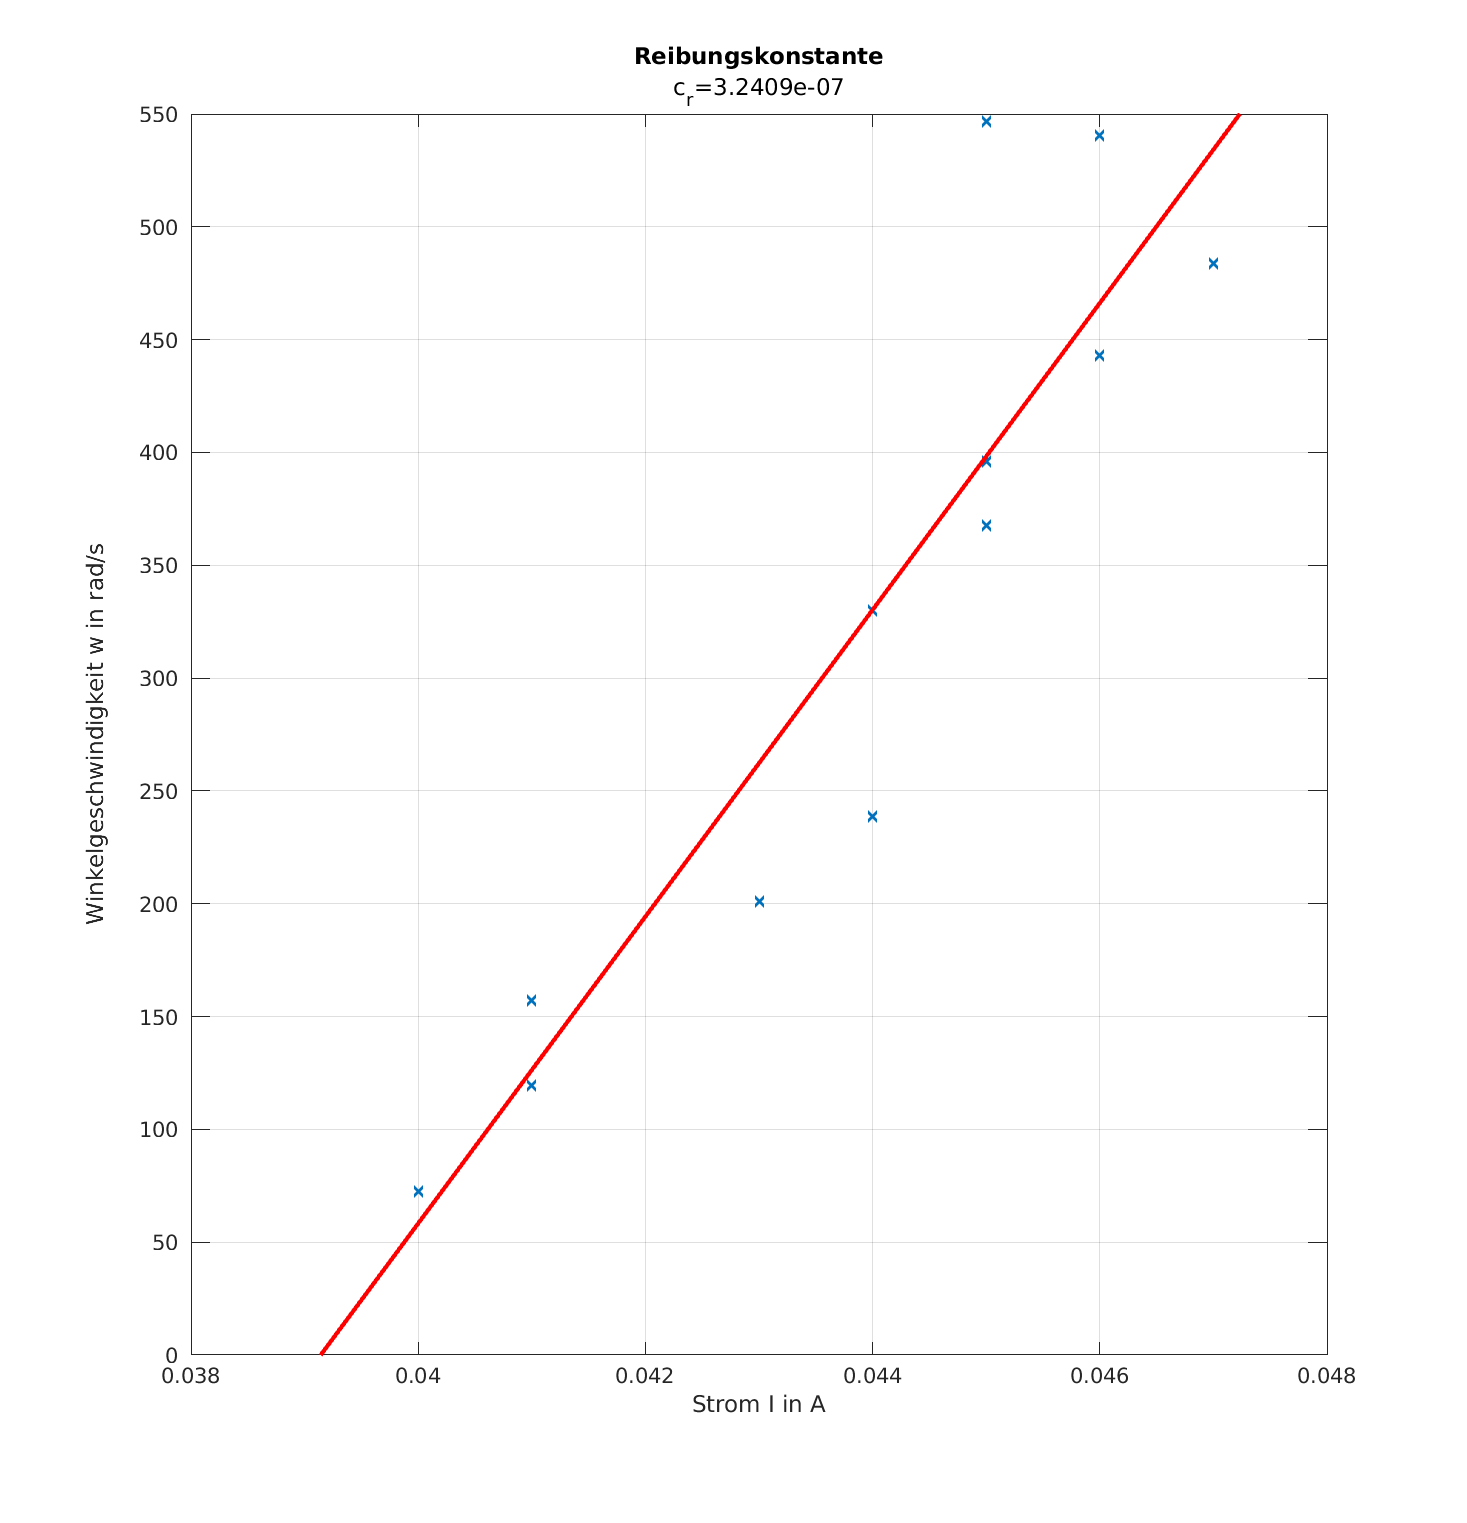
\includegraphics[width=1\textwidth]{as_labor02_2.png}
 \caption{Plot der Aufgabe 1}
 \label{fig:PlotAufgabe1}
\end{figure}